
%(BEGIN_QUESTION)
% Copyright 2011, Tony R. Kuphaldt, released under the Creative Commons Attribution License (v 1.0)
% This means you may do almost anything with this work of mine, so long as you give me proper credit

A pair of motor-driven compressors work in tandem to compress gas at an industrial ammonia production facility:

$$\includegraphics[width=15.5cm]{i00700x01.eps}$$

Explain how this control system attempts to evenly match the load between the two compressors, so that one is never working harder than the other, yet at the same time the two machines work together to maintain a common goal.

\vskip 80pt

Additionally, explain what will happen if flowmeter FT-235 fails with a low signal.

\vfil 

\underbar{file i00700}
\eject
%(END_QUESTION)





%(BEGIN_ANSWER)

This is a graded question -- no answers or hints given!

%(END_ANSWER)





%(BEGIN_NOTES)

The upper compressor's speed is cascade-controlled by discharge pressure.  The lower compressor's speed is cascade-controlled by flow.  Since the flow rate going into the upper compressor is used as the setpoint for the lower compressor's flow controller, the lower compressor will try to match flow in a 1:1 ratio.

\vskip 10pt

If FT-235 fails low, the lower compressor's flow controller will receive a remote setpoint of zero.  Thus, it will stop, placing all load on the upper compressor.  The upper compressor will then pick up speed in an attempt to maintain adequate discharge pressure.  The lower check-valve will prevent any of the upper compressor's discharge flow from ``back-flowing'' through the stopped lower compressor.

%INDEX% Control, strategies: ratio
%INDEX% Process: compressor load control

%(END_NOTES)


